 \section{Data processing approaches}\label{data-processing-approaches}
        
\subsection{Introduction}\label{data-processing-intro}

From the start of the project, our goal was to work on streaming data, piped in a continuous fashion to BMW's processing infrastructure. We encountered several challenges, which explains why we chose to handle data in various ways. Below is the timeline of the different solutions we came up with to deal with each problem:

\begin{enumerate}
    \item Since our BMW colleagues needed time to hand us their data, we came up with the idea of generating our own Flowlogs (\ref{flowlogs-stream-generation},\ref{fig:json_generator}). This allowed us not to loose time, but the generated data lacked the daily patterns of real-life data, so this approach was just temporary.
    \item Then, once the real-life data was delivered to us, we could train some models (DeepAR, RCF, MeanPredictor) on it (\ref{fixed-data-approach}), but were still lacking their streaming version.
    \item Indeed, we also wished to build tools able to process the original streaming data, but due to security concerns, we couldn't simply plug ourselves to BMW systems, and had to some extent write some tools mocking these data streams:\\
    \begin{itemize}
        \item We wrote a script generating a continuous stream from BMW's real-life data, in order to test the behavior of our whole processing pipeline (\ref{sec:streaming-data-approach})
        \item We also wanted to test how the RCF algorithm works on data streams, and for this we had to build a Kinesis-based pipeline(\ref{sec:real_time_anomaly_detection}).
    \end{itemize}
\end{enumerate}

\textbf{Keeping the evolution of the project in mind is important to understand the choices we made regarding the pipeline architecture.  \ref{data-processing-approaches}}
        
        \subsection{Data generation}
        \label{sec:data_generation}
        When it comes to data in Machine Learning models, in most cases the more training data there is, the better results we can achieve. Unfortunately in case of this project, we did not have the desired amount of data to get the appropriate results from the models. As a short term solution for this problem, the team decided to generate some data that has random anomaly spikes. The section below provides a description of data generation pipeline. \\
        \subsubsection{Flowlogs stream generation}\label{flowlogs-stream-generation}
        \textit{Author: Nursultan Shabykeev} \\
        
        Prior to getting real data from BMW, we decided to generate the data with random high anomaly peaks. We needed this artificial data to start training and testing our models.\\
        To implement this, we decided to write 2 types of services. The first one continuously generates sequential http-requests to the receiver, hereby, creating 'normal' behaviour of a system. The second one awakes randomly 2 times per day and sends multiple requests within several minutes. This leads to an anomaly situation. Figure \ref{fig:data-generation} demonstrates a pattern of our artificially generated data.
        
         \begin{figure}[h]
            \centering
            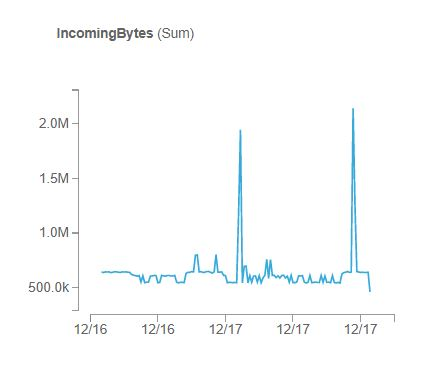
\includegraphics{images/data-generation.jpg}
            \caption{The pattern of the generated data}
            \label{fig:data-generation}
        \end{figure}
        \FloatBarrier
        
        \subsubsection{Architecture}
        After studying services that AWS offers for capturing continuous real-time data, we came to the following architecture. We placed two types of sender micro-services into separate EC2 instances within a common Amazon Virtual Private Cloud (VPC)\footnote{ https://docs.aws.amazon.com/vpc/index.html}. Our receiver is basically an EC2 instance within another VPC. In essence, VPC is a virtual network environment that enables a user to easily manage resources in it. One of its useful features is Flow Logs\footnote{ https://docs.aws.amazon.com/vpc/latest/userguide/flow-logs.html}. Flow Logs allows us to access information about all inbound and outbound traffic to and from instances in VPC. This information is represented in records. A record  consists of fields that describe the traffic flow and has the following format:
            \begin{figure}[h]
                \centering
                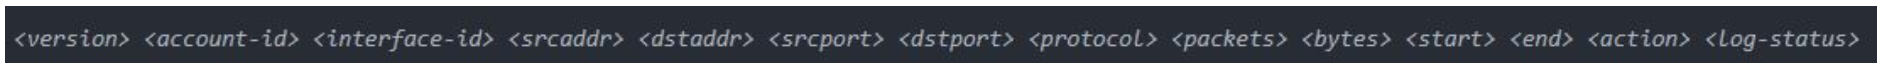
\includegraphics[width=1\textwidth]{images/flow-log-format.png}
                \caption{Flow Log record format}
                \label{fig:flow-log-format}
            \end{figure}
        \FloatBarrier
        
        In our case, we enabled Flow Logs for a receiver's VPC to capture requests from senders. We did not track responses from the receiver. Figure \ref{fig:data_generation_pipeline} shows a general pipeline for data generation. 
         \begin{figure}[h]
            \centering
            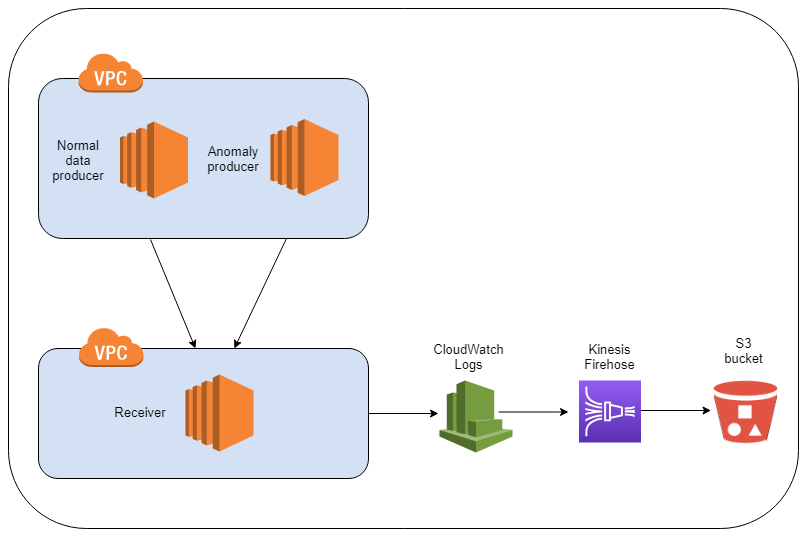
\includegraphics[width=0.8\textwidth]{images/data-generation-pipeline.png}
            \caption{Data generation pipeline}
            \label{fig:data_generation_pipeline}
        \end{figure}
        \FloatBarrier
        
        \subsubsection{Working with streaming data} 
        VPC Flow Logs can be published either to Amazon CloudWatch Logs or directly to Amazon S3. We decided to publish to CloudWatch Logs because later we would like to try out Kinesis real-time data analysis services from AWS on the streaming log data. 
        Amazon Kinesis Data Streams (KDS) is a set of services provided by AWS to work with real-time streaming data: 
        \begin{displayquote}
            Amazon KDS is a massively scalable and durable real-time data streaming service. KDS can continuously capture gigabytes of data per second from hundreds of thousands of sources. . . . The data collected is available in milliseconds to enable real-time analytics use cases. . . .\cite{awsKds} 
        \end{displayquote} 
        From this set of services, we used Kinesis Firehose to load VPC Flow Logs. Creation of a Firehose delivery stream can be done as follows, replacing the placeholder values for RoleARN and BucketARN with the role and S3 bucket ARN where flog logs will be stored:
        \begin{figure}[h]
            \centering
            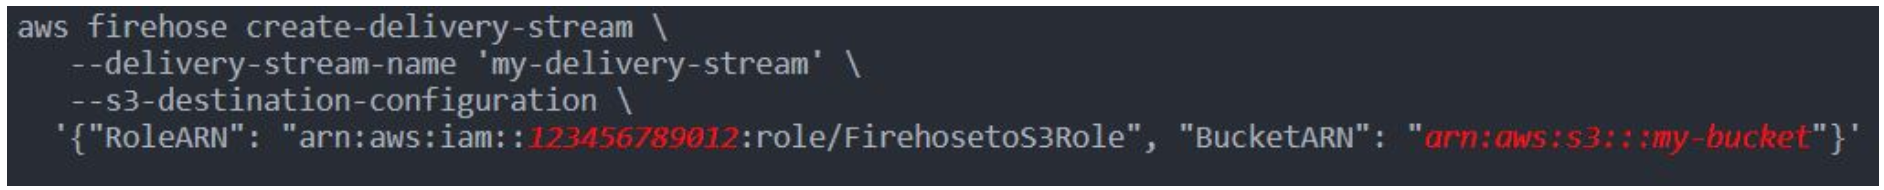
\includegraphics[width=1\textwidth]{images/kinesis-firehose.png}
            \caption{Creation of Kinesis Data Firehose delivery stream}
            \label{fig:kinesis_firehose_delivery}
        \end{figure}
        \FloatBarrier
        
        After the Firehose delivery stream is ready and in an active state, we direct the streaming data to it from CloudWatch Logs. This can be done through a subscription filter\footnote{ https://docs.aws.amazon.com/AmazonCloudWatch/latest/logs/SubscriptionFilters.html}. The subscription filter connects a Firehose stream and CloudWatch logs and starts a flow of real-time log data to a Firehose delivery stream.
        \begin{figure}[h]
            \centering
            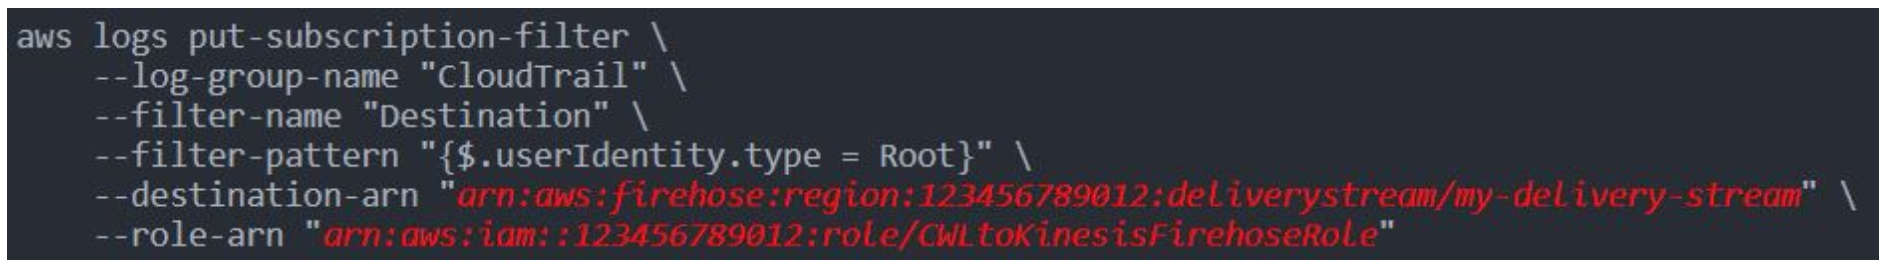
\includegraphics[width=1\textwidth]{images/subscription-filter-creation.png}
            \caption{Creation of subscription filter}
            \label{fig:subscription_filter_creation}
        \end{figure}
        \FloatBarrier    
        After the subscription filter is set up, CloudWatch Logs sends all the incoming log events that match the filter pattern to Amazon Kinesis Data Firehose delivery stream. It might take a few minutes before the data will be saved into S3. However, it is possible to monitor a size of incoming data and other metrics in a \textit{Monitoring} tab in a Firehose console page. \\
        While creating the subscription filter, it is important to define properly IAM roles and permission policies and correctly associate the permissions policy with the role. The full description of establishing the connection between Kinesis streams and CloudWatch Logs is available in an official documentation \cite{awsFirehoseSubFilter}.\\
        As stated above, we used Kinesis services to get introduced to real-time data analysis tools available in AWS. Later, we installed Kinesis Data Analytics\footnote{https://aws.amazon.com/kinesis/data-analytics} as a before step before sending the data to S3 bucket (see figure \ref{fig:data_generation_pipeline}). This way we tried to make a simple analysis and, for the first time, apply Random Cut Forest algorithm to the artificially streamed data. Even though, the work described in the current section was a temporary implementation, it generally helped us to come up later with final solutions.\\
        As the real data was eventually published in an S3 bucket, we did not need the data generation pipeline anymore. That is why we currently do not deliver it, only the code for generating requests is available in GitHub. The version that is implemented in Java is available in: \lstinline{utils/flowlogs-stream-generation/}.\\
        Another approach that is implemented in Python is described in the following section.
      
        \subsubsection{Data Generator - Python }\label{data-generator}
        
        \textit{Author: Ali Karaki}

        The Dummy Data Generator in Python variant is an alternative version of the one being discribed above. It simulates a stream of https requests to a specific IP (EC2 instance inside a VPC). It is highly configurable from scheduled time for requests, has a dynamic server IP for the EC2 instance, and a placeholder for the number of desired requests being sent. We needed an easy to customize script that can generate data fast. This script fulfills this requirement. It had no complex dependencies and has a pretty fast executions.\\ In concept, the workflow to generate dummy data was to do the following:
            \begin{enumerate}
                \item It sends HTTPS requests with our scripts to an EC2 instance.
                \item The logs from EC2 instance are saved in CloudWatch.
                \item VPC Flowlogs are saved inside a bucket on S3.
                \item Flowlogs aggregator lambda function is used to aggregate all the files into actual data set.
            \end{enumerate}
        A request may be rejected or accepted when it reached the EC2, by comparing it to the IP of a machine from the VPC (it can be seen in Fig. \ref{fig:data_gen}).
        \begin{figure}[h!]
            \centering
            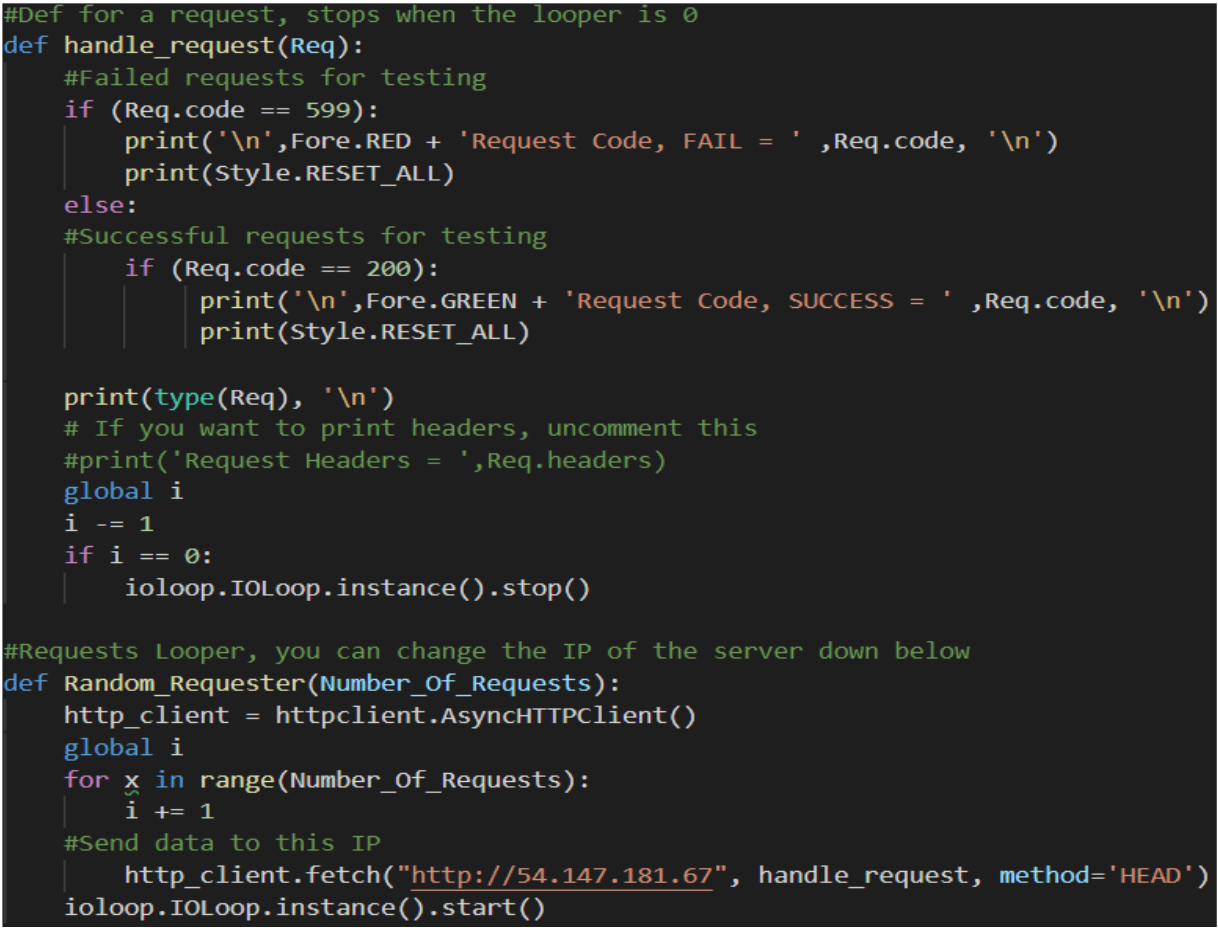
\includegraphics[width=1\textwidth]{images/data-gen-2.png}
            \caption{Data generation in a python script}
            \label{fig:data_gen}
        \end{figure}\\
        Requests are sent to a specific IP, the requests are categorized into 2 sections: successful and failed with codes 200 and 599 respectively.\\
        The sent data, that is already separated into successful and failed requests, and the number of requests are the variables used for anomaly detection.\\
        Anomalies detected with this data correspond to the number of requests recorded in a specific timestamp. So the code logic goes as following:
        \begin{enumerate}
    \item Send failed requests and successful requests to the EC2 instance
    \item Randomly send those requests in 2 different methods
    \item Every day from Monday to Sunday, randomly send only 1 very abnormal number of requests and 1 very high number of requests
\end{enumerate}
  
        As this script is used only to generate the data the script runs in an infinite loop until it is disabled manually, with a possibility to configure the number of requests and date of sending them.\\


\subsection{Fixed data approach}\label{fixed-data-approach}
    %Author: Marius
\label{sec:fixed_data}
\textit{Author: Marius Schidlack} \\
After working with our fake data streams for some time, we were provided with some real data by BMW. The data was presented in two different formats: Flowlogs and Metrics. They contained network traffic information  starting from December 21, 2018. 
Flowlogs contain raw information about network traffic, e.g. which IP-adress made a request to which server at what time along with other details.

In this section, we will focus on how we used the Metrics files. The Metrics already accumulate the raw network traffic data from the Flowlogs and only contain information about the number of requests. More specifically, they contain the number of successful requests (with HTTP-Code 200) and failed requests (HTTP-Code 4xx and 5xx) at a certain time. Although the files were named \textit{output-mass.json}, they were not correctly encoded in JSON format. An example entry from one of the files can be seen in \ref{lst:metrics_example}.

\begin{minipage}{\linewidth}
\begin{lstlisting}[caption={Example entry from metrics data},label={lst:metrics_example}]
{
    [...]
    'response-code-4xx': {
    [...]
        'Datapoints': [
            {'Timestamp': datetime.datetime(2018, 12, 15, 11, 20, tzinfo=tzlocal()), 
            'SampleCount': 6.0, 
            'Unit': 'None'
            }
        ]
    }
}
\end{lstlisting}
\end{minipage}

For this reason (invalid JSON format) we had to write a custom python script to parse the data (i.e. to read the data from the files and load them into python objects). Once all the files are parsed, we take the \textit{SampleCount} values for each entry, and sort them into buckets according to their \textit{Timestamp}. For the time being, we did not differentiate between successful or failed requests, however, this might be a useful thing to do in the future. The buckets were chosen to be of 5 minute granularity in the final product, however we also experimented with 1 minute buckets.
\begin{figure}[h]
    \centering
    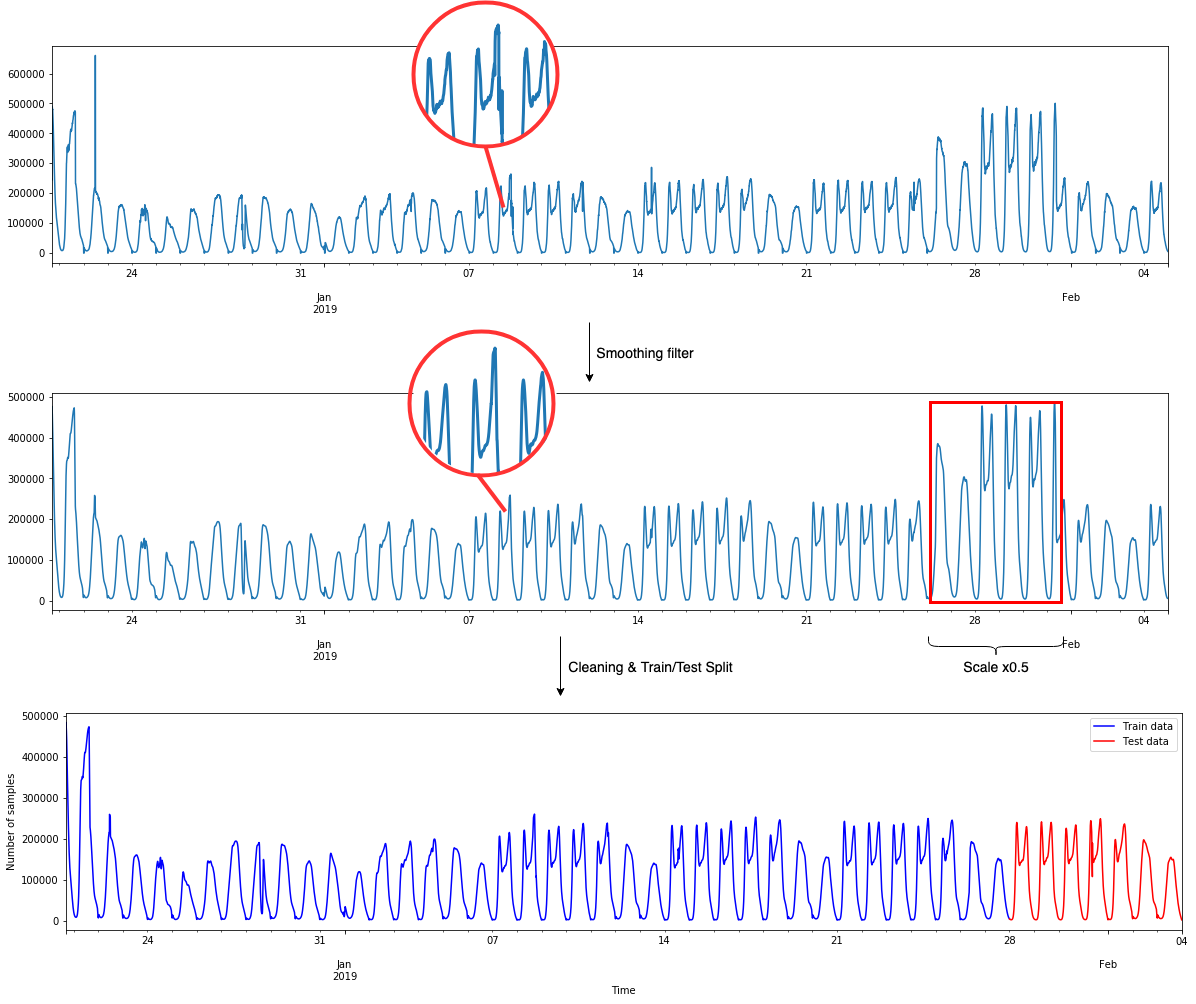
\includegraphics[width=1\textwidth]{images/data_preprocessing.png}
    \caption{Data preprocessing pipeline}
    \label{fig:data_preprocessing}
\end{figure}
\afterpage{\FloatBarrier}
A smaller bucket size means higher responsiveness in a real time anomaly detection model, since in order to react to incoming data, we have to wait until the current bucket is full. On the other hand, if the bucket size gets too small, the machine learning model might get vulnerable to noise in the data. Larger buckets means less number of buckets and compress the training data which allows to train the model faster. Furthermore this can make the model more robust to noisy data. \\
Next, we summed up the values in every bucket to obtain the raw time series, which can be seen in figure \ref{fig:data_preprocessing} in the first graph. 
\subsubsection{Preprocessing and Cleaning}
We noticed that the data is still very noisy and contains some impurities. For example, the data between the 26th and the 31st of January was scaled up by a factor of two for unknown reasons (see red box in the second graph in figure \ref{fig:data_preprocessing}).
We reduced the noise by applying a smoothing convolution to the data, and scaled down the aforementioned scaled up time interval (cf. fig. \ref{fig:data_preprocessing}).
One might argue that in time series data, the value of one point in time is highly correlated to the previous ones. Smoothing the time series exploits this property to get rid of sudden and unexpected jumps in the training data, or in other words, we reduce outliers and make training of our machine learning models more robust.
Finally, we separated one week of data and defined it as out test set.
\subsubsection{Exporting for Machine Learning Models}
For further use with the Machine Learning models described later, the data had to exported in different formats. For the Random Cut Forest and the Mean Predictor, the data can be provided in a simple CSV format with \textit{Timestamp} and \textit{Value}. The DeepAR Model however requires a more complex format which is described in more detail in chapter \pageref{ch:deepar}.

\subsubsection{Advantages and Disadvantages}
While extracting the data from the Metrics files is convenient and simple, this approach has drawbacks: we have no control over how the Metrics files are accumulated. In order to obtain full control over the data stream, one must work with the raw Flowlogs files. An approach that utilizes the Flowlogs data from scratch is described in section \ref{sec:real_time_anomaly_detection}.


    
\subsection{Streaming data approach}
\textit{Author: Alexandre Rozier} 
\label{sec:streaming-data-approach}
    This approach uses \textbg{ a custom script hosted on EC2} \label{ec2script}.
    \textbf{Code relative to this section can be found in \lstinline{utils/streaming-data-mock.py}}. \\
    Since we were just provided with a fixed dataset and did not have access to the real BMW data stream, we had to create our own mock of it, to test our solution with real-time data. Its principle is quite simple: we extract one default week from the fixed dataset provided by BMW, and use a script to send over and over this particular week on our AWS infrastructure. \par
    
    An EC2 instance is spun up via Terraform (\ref{ec2-tf}), then provisioned thanks to an Ansible script (installation of the correct python version, required dependencies,  upload of the source code and execution). \par
    
    To be more specific, the script triggers a job every 15 minutes, charged with uploading a new batch of data to a specific entry point on AWS S3.
    Please note that the data is sent synchronously with the current time, that is, at 8am we will send data concerning the timespan 7:45-8:00am from the default week. \par
    
    We chose to implement this fake stream in order to test the whole pipeline, because it was the closest we could imitate BMW's infrastructure putting new batches of data to our entry S3 bucket. This was useful during the final presentation (where we could show our pipeline processing live data), and also to work as close a possible to a real-life scenario.

% https://www.overleaf.com/2386286181cpqpvxpvkkzt